Como dito anteriormente, a representação pelas $\delta$-coordenadas permitem o encapsulamento de informações locais da superfície. Além disso, as matrizes $L, L_s$ e $D$ utilizadas são esparsas, e computacionalmente mais eficientes em questão de memória e tempo de execução.

Com isso, a modelagem utilizando estas coordenadas possuem algumas vantagens interessantes, que serão exploradas nos próximos tópicos.

\subsection{Representação eficiente de formas}

A primeira grande aplicação das coordenadas diferenciais a ser analisada é a representação eficiente de formas, mesmo ao utilizar informações reduzidas do domínio. Se utilizada uma boa base para representação, é necessária apenas uma parcela da função de base para representar toda a geometria \cite{sorkine2004}.

Desta forma, com apenas informações de conectividade da malha e alguns pontos fixados (denominados vértices âncora), é possível aproximar toda a geometria, a partir da resolução do sistema pelo método dos mínimos quadrados:

\begin{equation}\label{eq:sisrecover2}
\left( \frac{L}{\omega I_{m \times m} | 0} \right) \mathbf{x'} = \begin{pmatrix}
0\\
\omega\ c_{1:m}^{(x)}
\end{pmatrix}
\end{equation}

\noindent em que $c = \{v_1, v_2, \dots, v_m\}$ são os pontos âncora escolhidos como amostra, e $\omega > 0$ é o peso de cada restrição (assim como na equação \ref{eq:sisrecover}).

Da mesma forma que anteriormente, de forma gráfica, para facilitar a visualização do sistema:

\begin{center}
	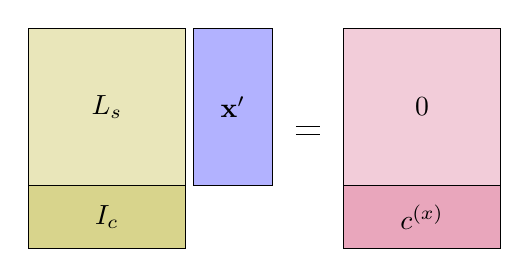
\begin{tikzpicture}
	\filldraw[fill=olive!20!white, draw=black] (0,0) rectangle node{$L_s$} (2,2);
	\filldraw[fill=olive!35!white, draw=black] (0,0) rectangle node{$I_c$} (2,-0.8);
	\filldraw[fill=blue!30!white, draw=black] (2.1,0) rectangle node{$\mathbf{x}'$} (3.1,2);
	\draw (3.4, 0.65) -- (3.7, 0.65);
	\draw (3.4, 0.75) -- (3.7, 0.75);
	\filldraw[fill=purple!20!white, draw=black] (4,0) rectangle node{$0$} (6,2);
	\filldraw[fill=purple!35!white, draw=black] (4,0) rectangle node{$c^{(x)}$} (6,-0.8);
	\end{tikzpicture}
\end{center}

As figuras \ref{fig:ex1rep} e \ref{fig:ex2rep} mostram exemplos de representação de curvas parametrizadas a partir de uma parcela dos pontos originais.

\begin{figure}[htb]
	\centering
	\begin{subfigure}[b]{0.43\textwidth}
		\centering
		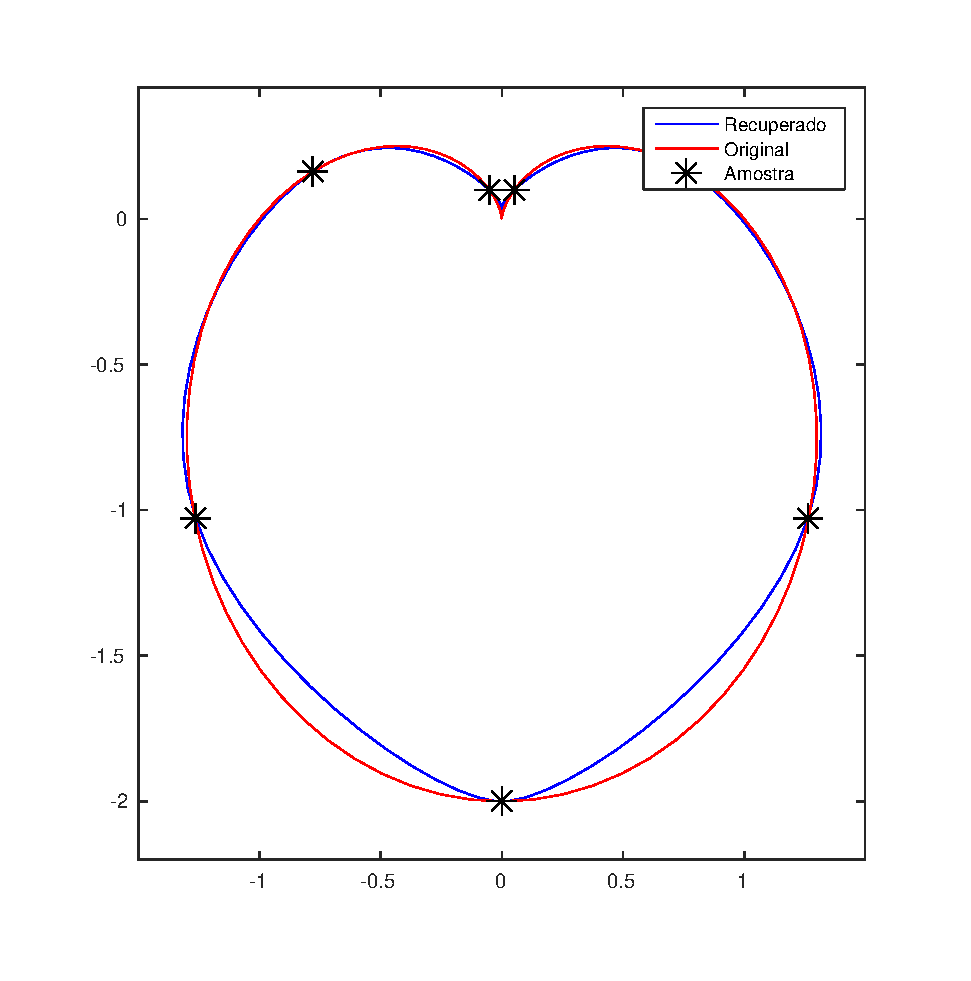
\includegraphics[width=\textwidth]{imagens/cap4/rep_1_8.eps}
		\caption{8 pontos}
		\label{fig:ex11}
	\end{subfigure}
	\hfill
	\begin{subfigure}[b]{0.43\textwidth}
		\centering
		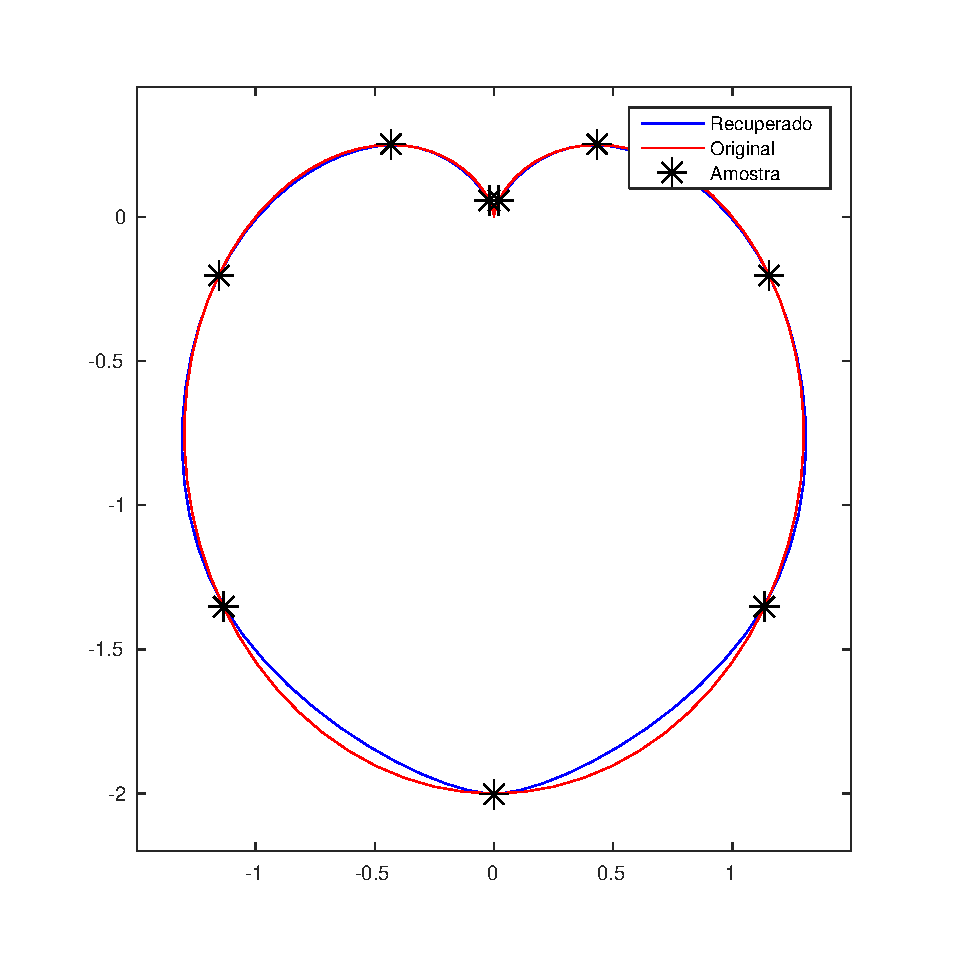
\includegraphics[width=\textwidth]{imagens/cap4/rep_1_10.eps}
		\caption{10 pontos}
		\label{fig:ex14}
	\end{subfigure}
	\hfill
	\begin{subfigure}[b]{0.43\textwidth}
		\centering
		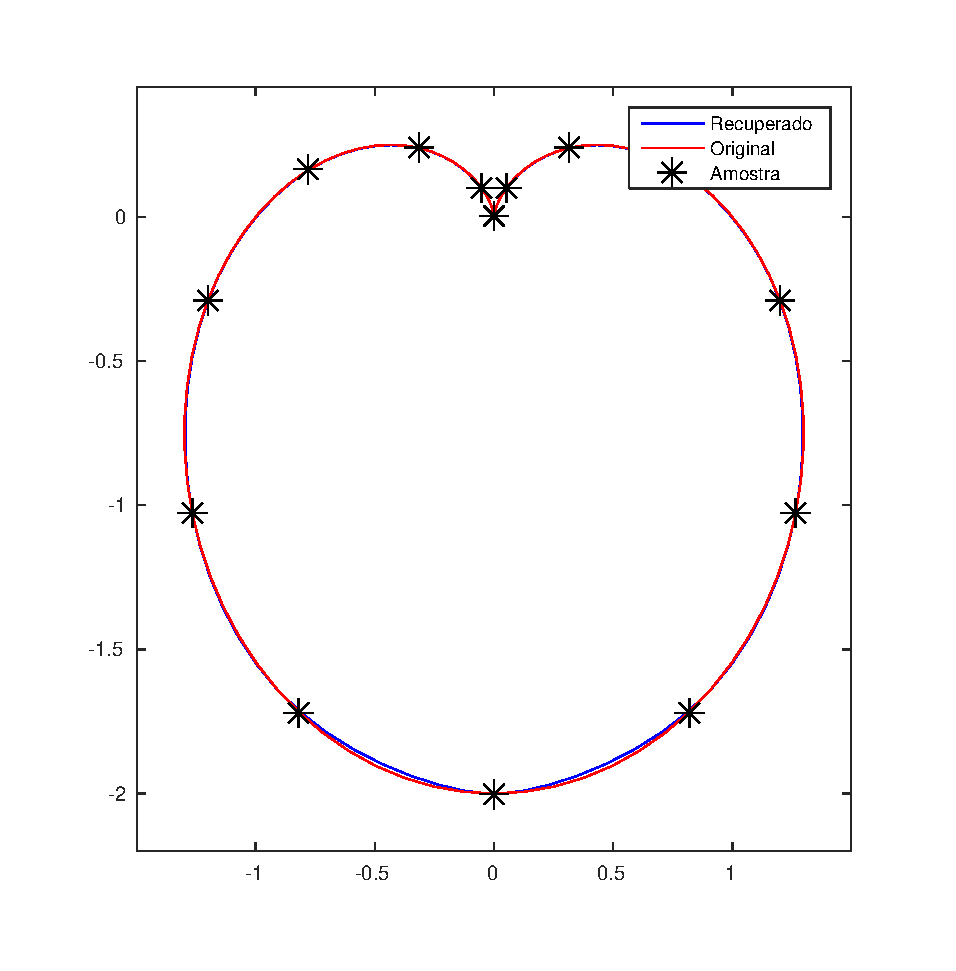
\includegraphics[width=\textwidth]{imagens/cap4/rep_1_15.eps}
		\caption{15 pontos}
		\label{fig:ex12}
	\end{subfigure}
	\hfill
	\begin{subfigure}[b]{0.43\textwidth}
		\centering
		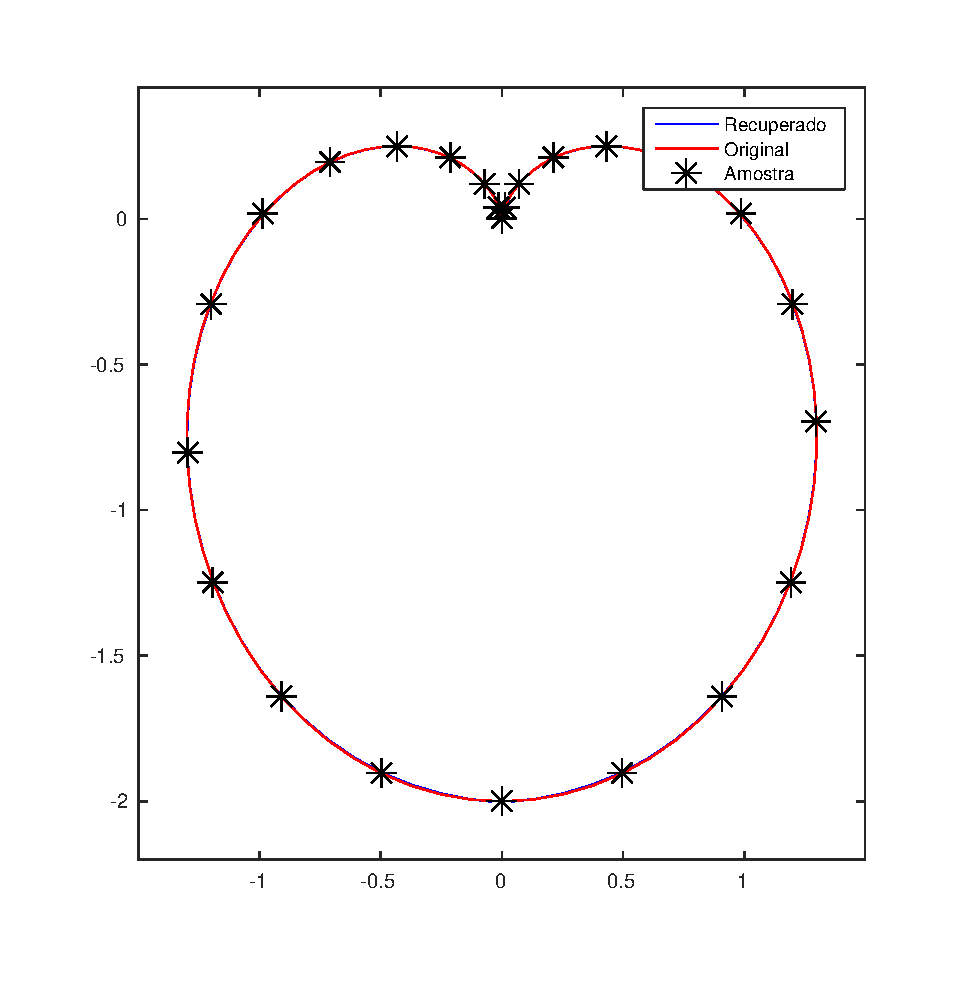
\includegraphics[width=\textwidth]{imagens/cap4/rep_1_25.eps}
		\caption{25 pontos}
		\label{fig:ex13}
	\end{subfigure}
	\caption{Representação da função paramétrica $(x(t), y(t)) = (sin(t) + 0.5 sen(2t), -cos(t) - 0.5 - 0.5 cos(2t))$ utilizando alguns pontos igualmente espaçados como amostra.}
	\label{fig:ex1rep}
\end{figure}


\begin{figure}[htb]
	\centering
	\begin{subfigure}[b]{0.43\textwidth}
		\centering
		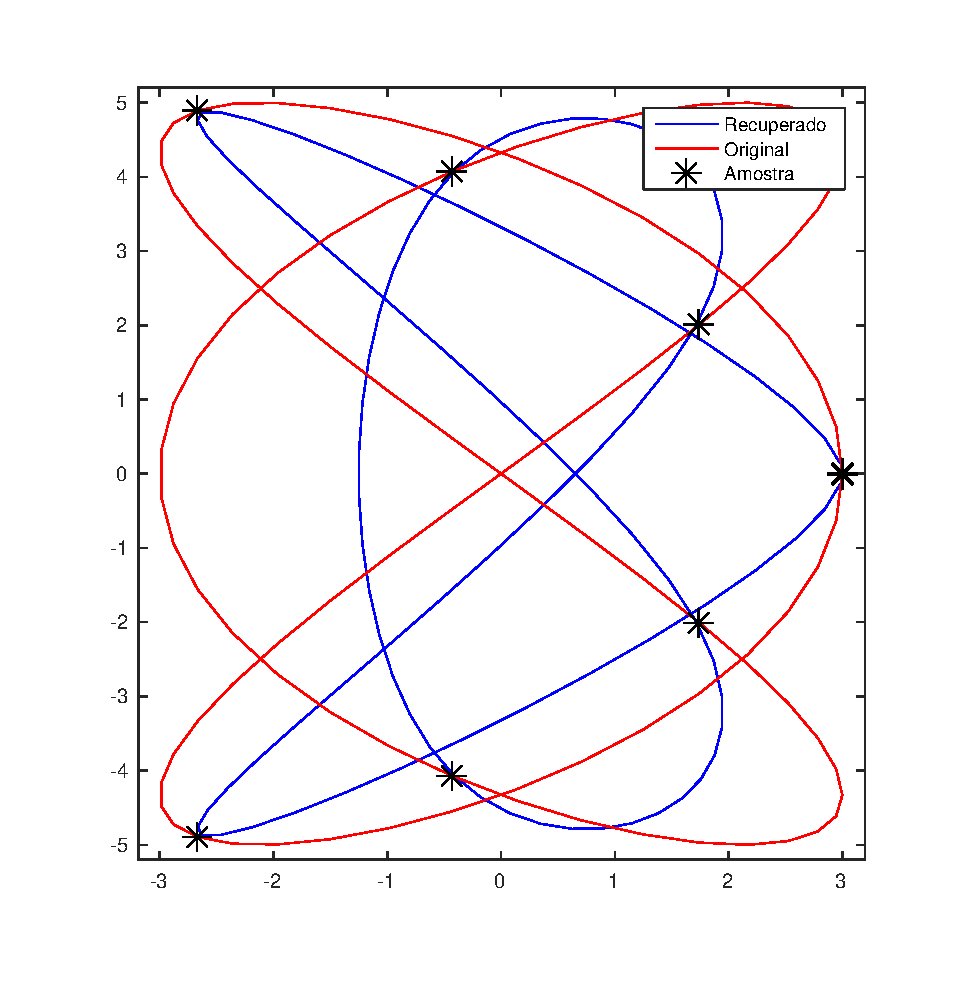
\includegraphics[width=\textwidth]{imagens/cap4/rep_2_8.eps}
		\caption{8 pontos}
		\label{fig:ex21}
	\end{subfigure}
	\hfill
	\begin{subfigure}[b]{0.43\textwidth}
		\centering
		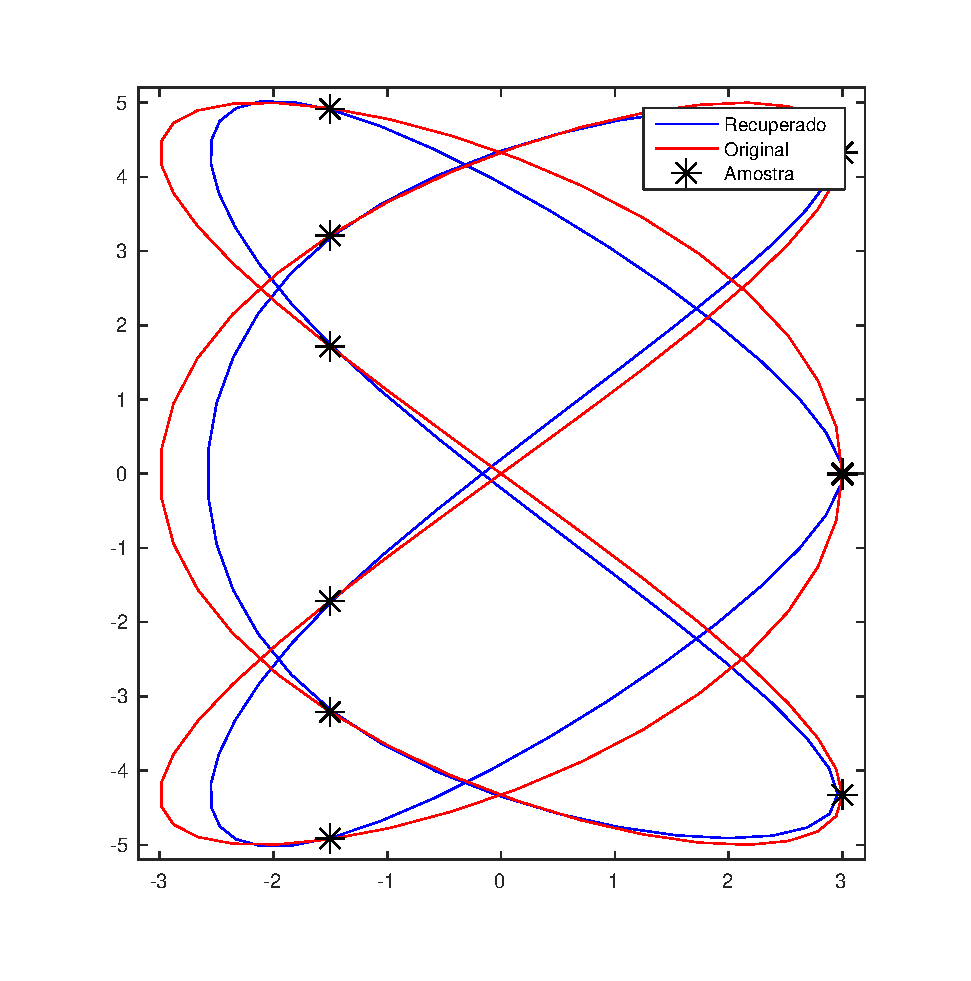
\includegraphics[width=\textwidth]{imagens/cap4/rep_2_10.eps}
		\caption{10 pontos}
		\label{fig:ex24}
	\end{subfigure}
	\hfill
	\begin{subfigure}[b]{0.43\textwidth}
		\centering
		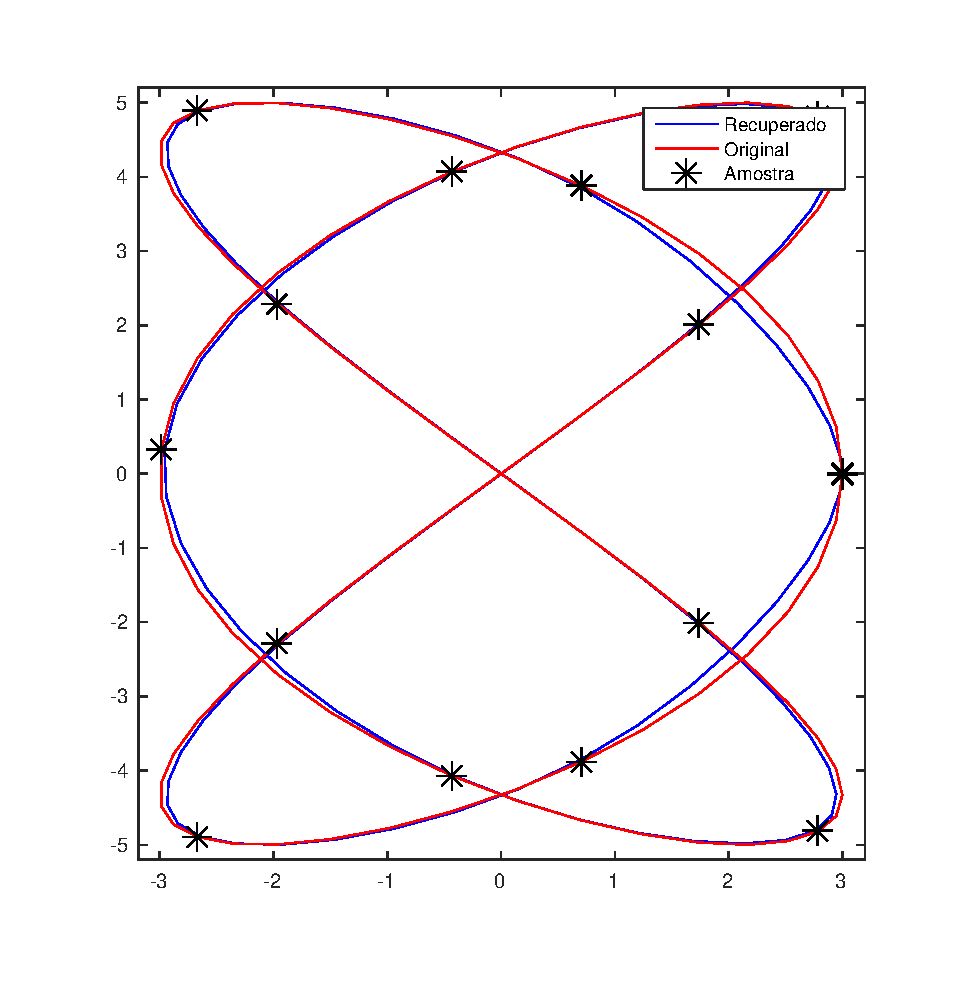
\includegraphics[width=\textwidth]{imagens/cap4/rep_2_15.eps}
		\caption{15 pontos}
		\label{fig:ex22}
	\end{subfigure}
	\hfill
	\begin{subfigure}[b]{0.43\textwidth}
		\centering
		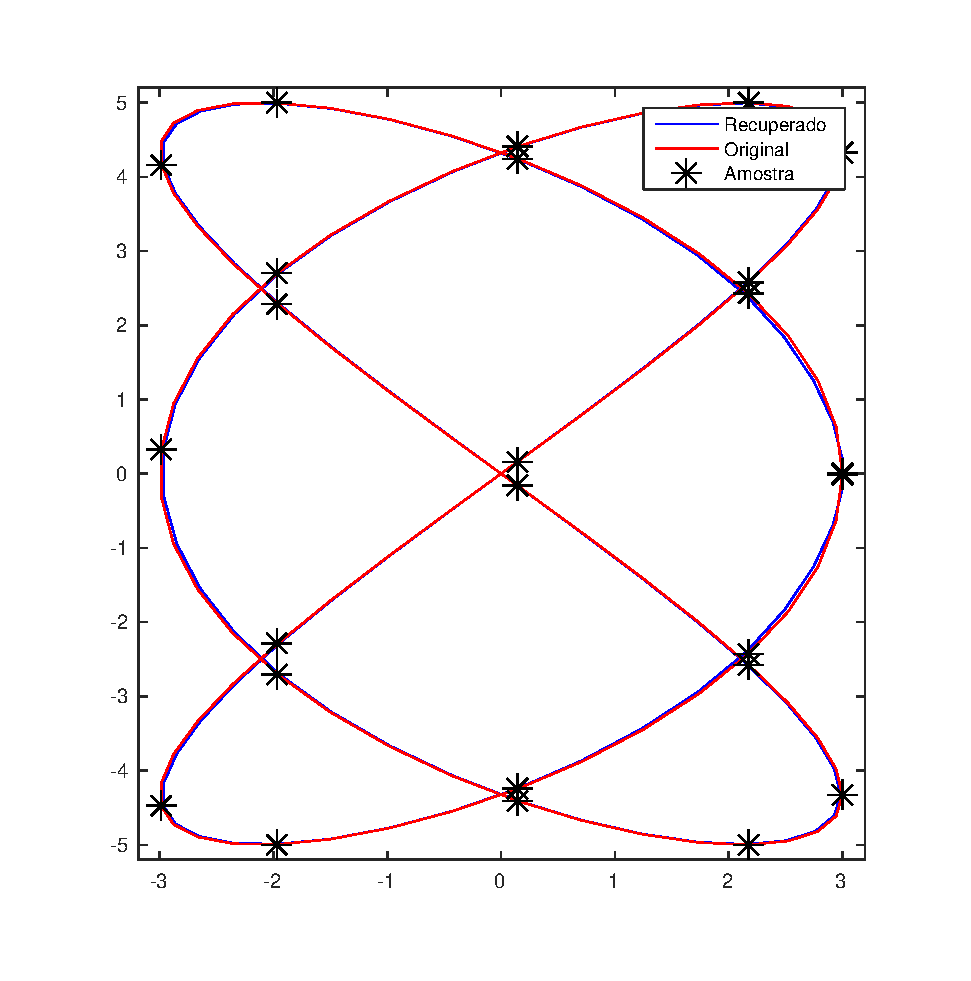
\includegraphics[width=\textwidth]{imagens/cap4/rep_2_25.eps}
		\caption{25 pontos}
		\label{fig:ex23}
	\end{subfigure} %[3 * cos(3 * t); 5 * sin(2 * t)]';
	\caption{Representação da função paramétrica $(x(t), y(t)) = (3 cos(3t), 5sen(2t))$ utilizando alguns pontos igualmente espaçados como amostra.}
	\label{fig:ex2rep}
\end{figure}

Um exemplo de representação de superfícies pode ser visto na figura \ref{fig:ex3rep}, também utilizando alguns pontos igualmente espaçados como amostra (âncora).

\begin{figure}[H]
	\centering
	\begin{subfigure}[b]{0.48\textwidth}
		\centering
		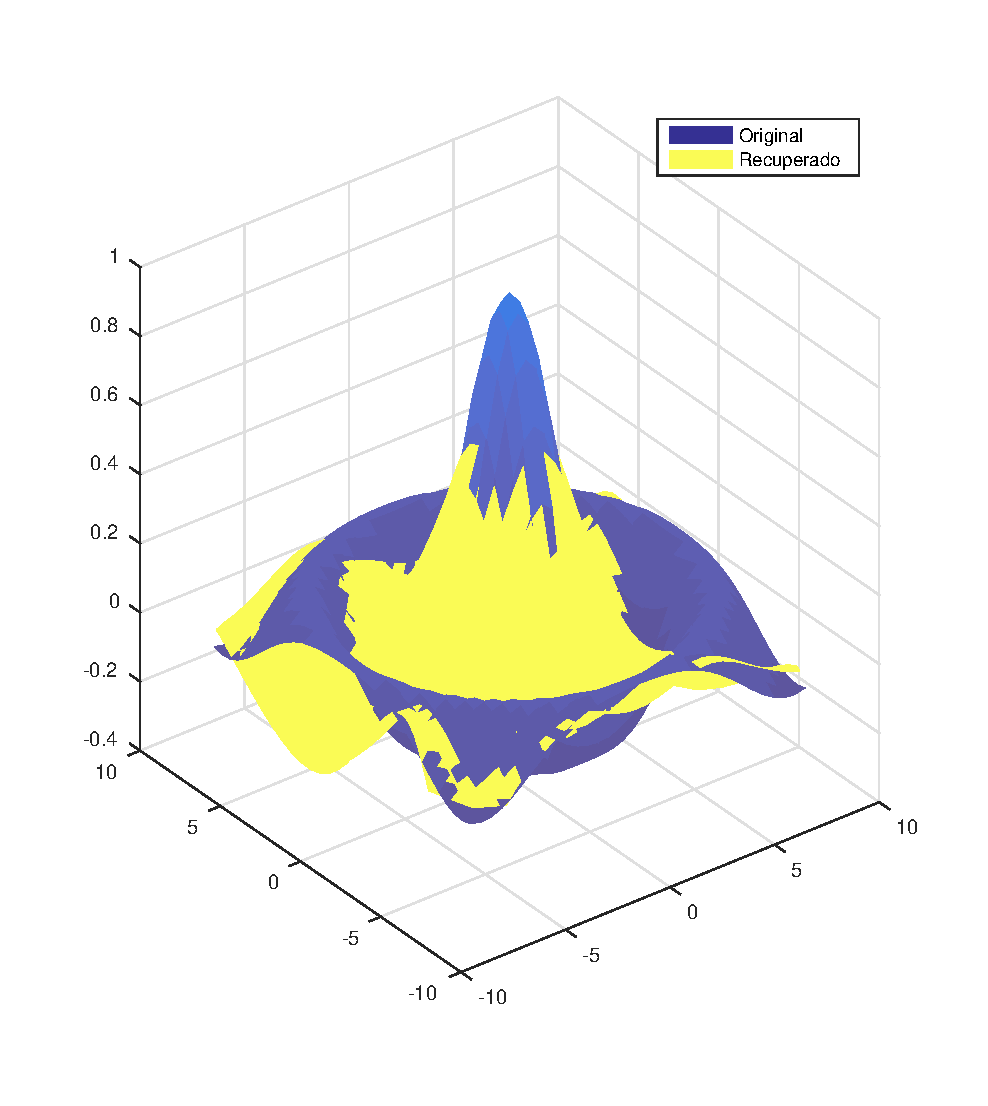
\includegraphics[width=\textwidth]{imagens/cap4/rep3_50.eps}
		\caption{50 pontos}
		\label{fig:ex31}
	\end{subfigure}
	\hfill
	\begin{subfigure}[b]{0.48\textwidth}
		\centering
		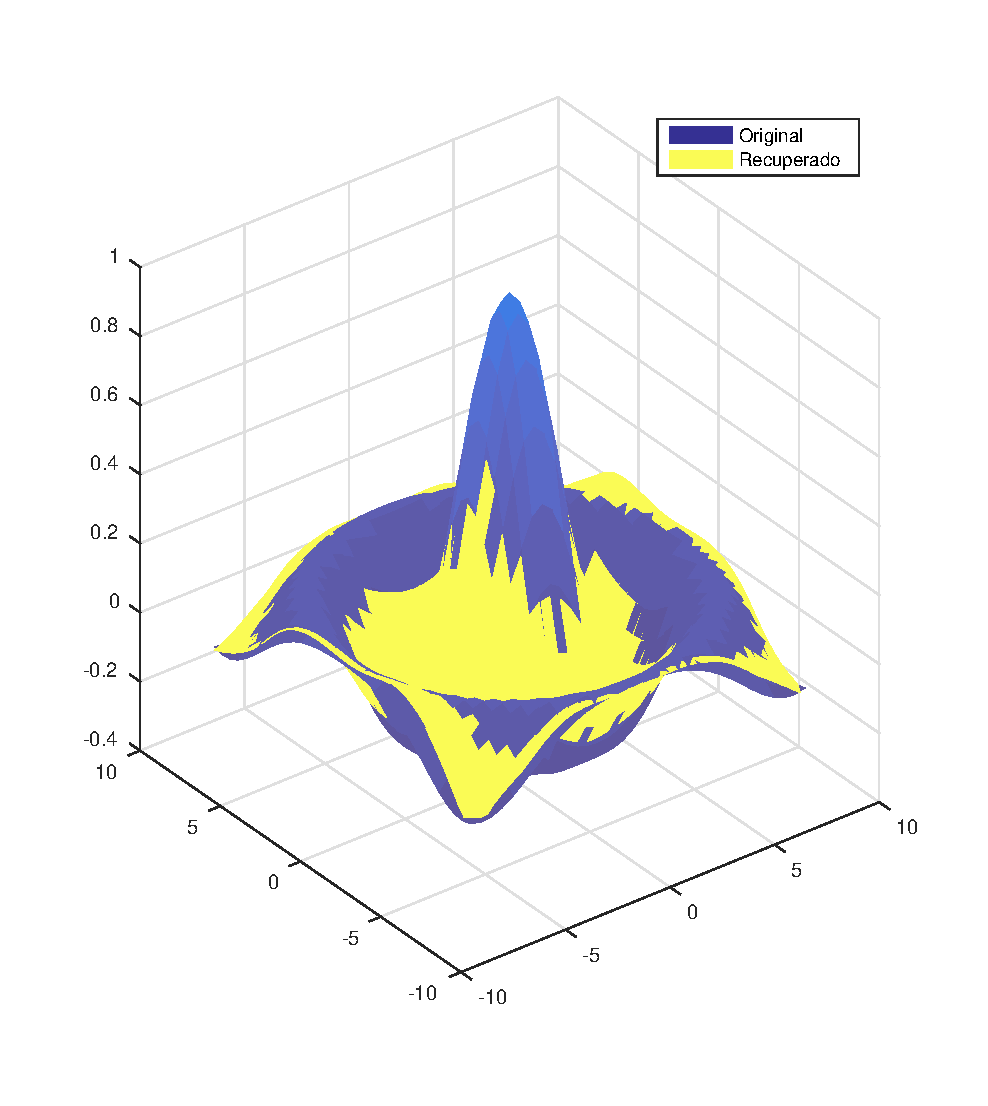
\includegraphics[width=\textwidth]{imagens/cap4/rep3_200.eps}
		\caption{200 pontos}
		\label{fig:ex32}
	\end{subfigure}
	\caption{Representação da função $z(x, y) = \frac{sen (\sqrt{x^2 + y^2})}{\sqrt{x^2 + y^2}}$ utilizando alguns pontos igualmente espaçados como amostra.}
	\label{fig:ex3rep}
\end{figure}

Outro exemplo em espaços tridimensionais pode ser visto na seguinte malha da figura \ref{fig:ex4rep}, utilizando alguns pontos (com índices igualmente espaçados) como âncoras:

\begin{figure}[H]
	\centering
	\begin{subfigure}[b]{0.47\textwidth}
		\centering
		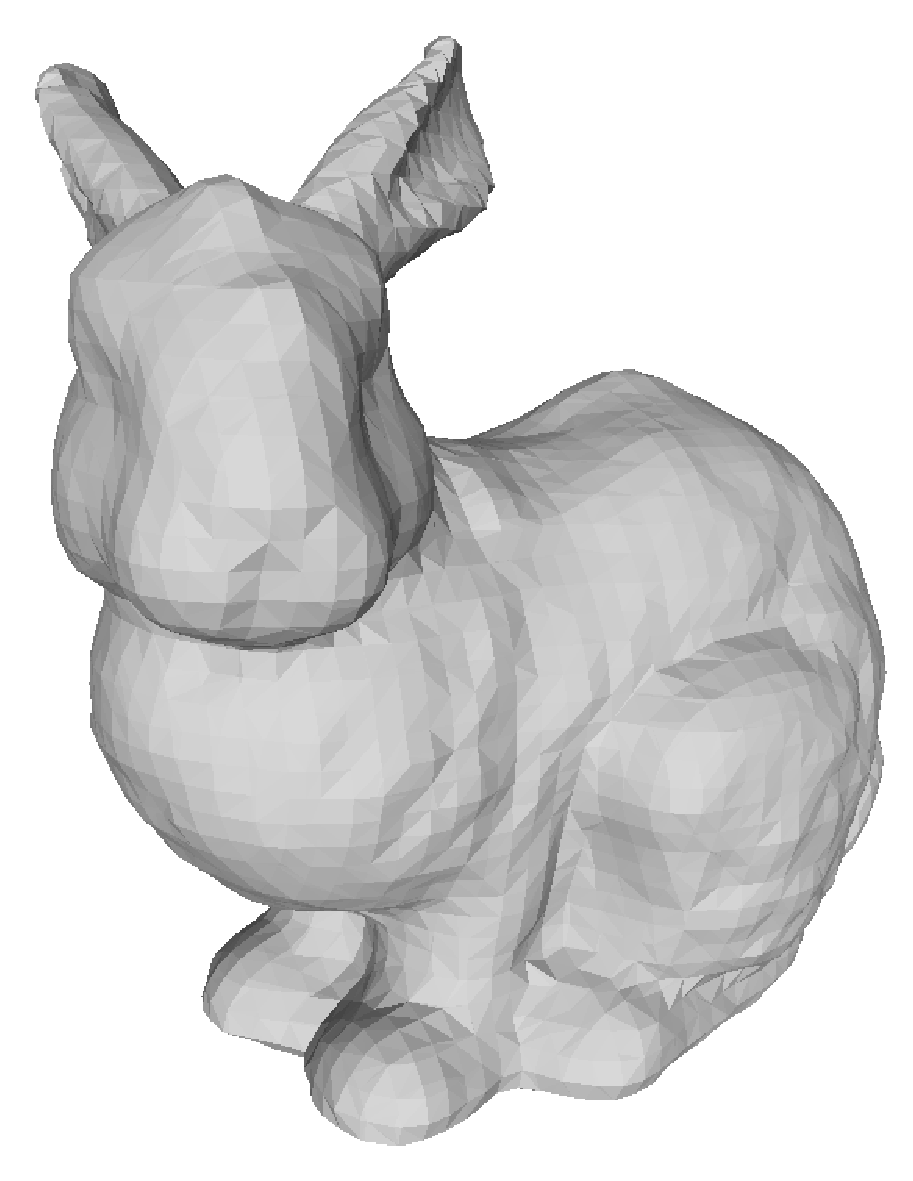
\includegraphics[width=\textwidth]{imagens/cap4/bunny_all.eps}
		\caption{Malha original}
		\label{fig:ex41}
	\end{subfigure}
	\hfill
	\begin{subfigure}[b]{0.47\textwidth}
	\centering
	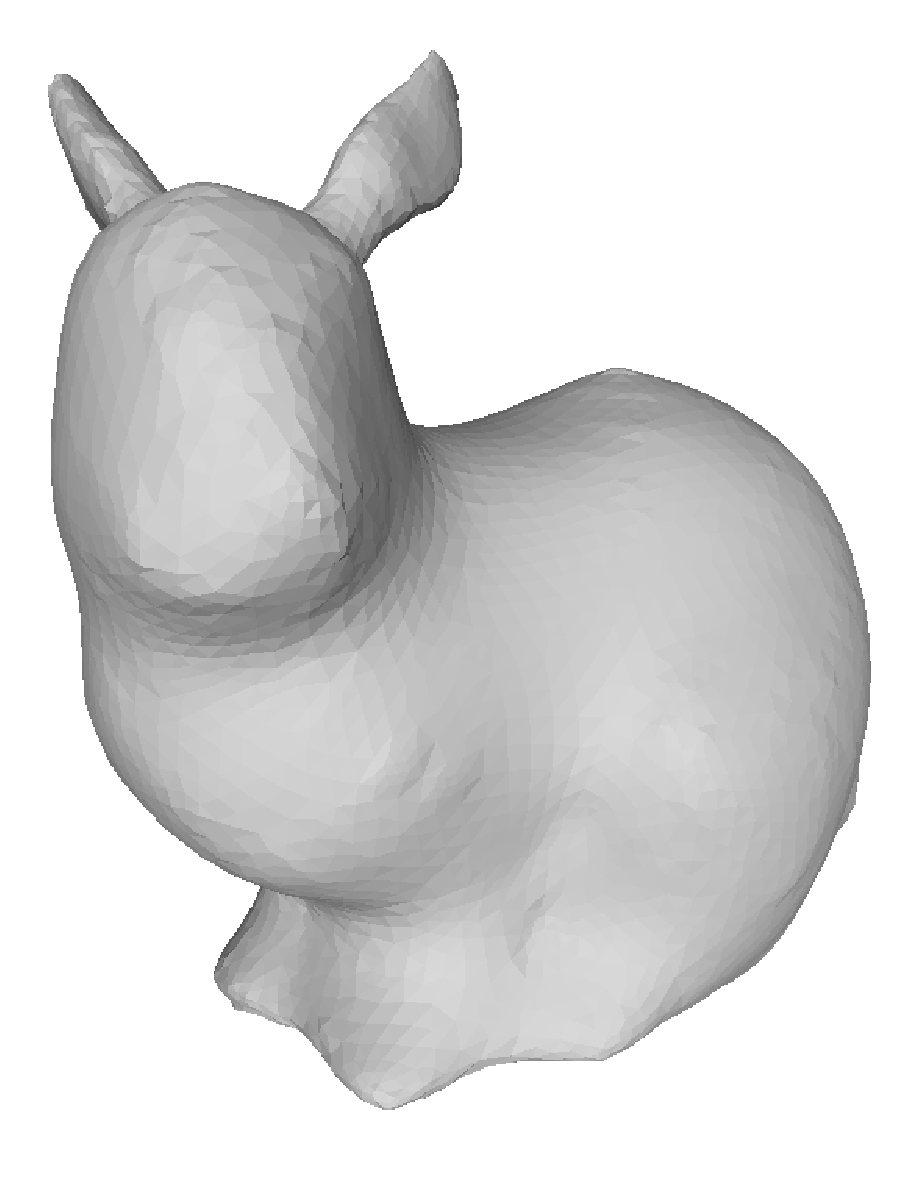
\includegraphics[width=\textwidth]{imagens/cap4/bunny_10.eps}
	\caption{10\% dos pontos}
	\label{fig:ex42}
	\end{subfigure}
	\\
	\begin{subfigure}[b]{0.47\textwidth}
		\centering
		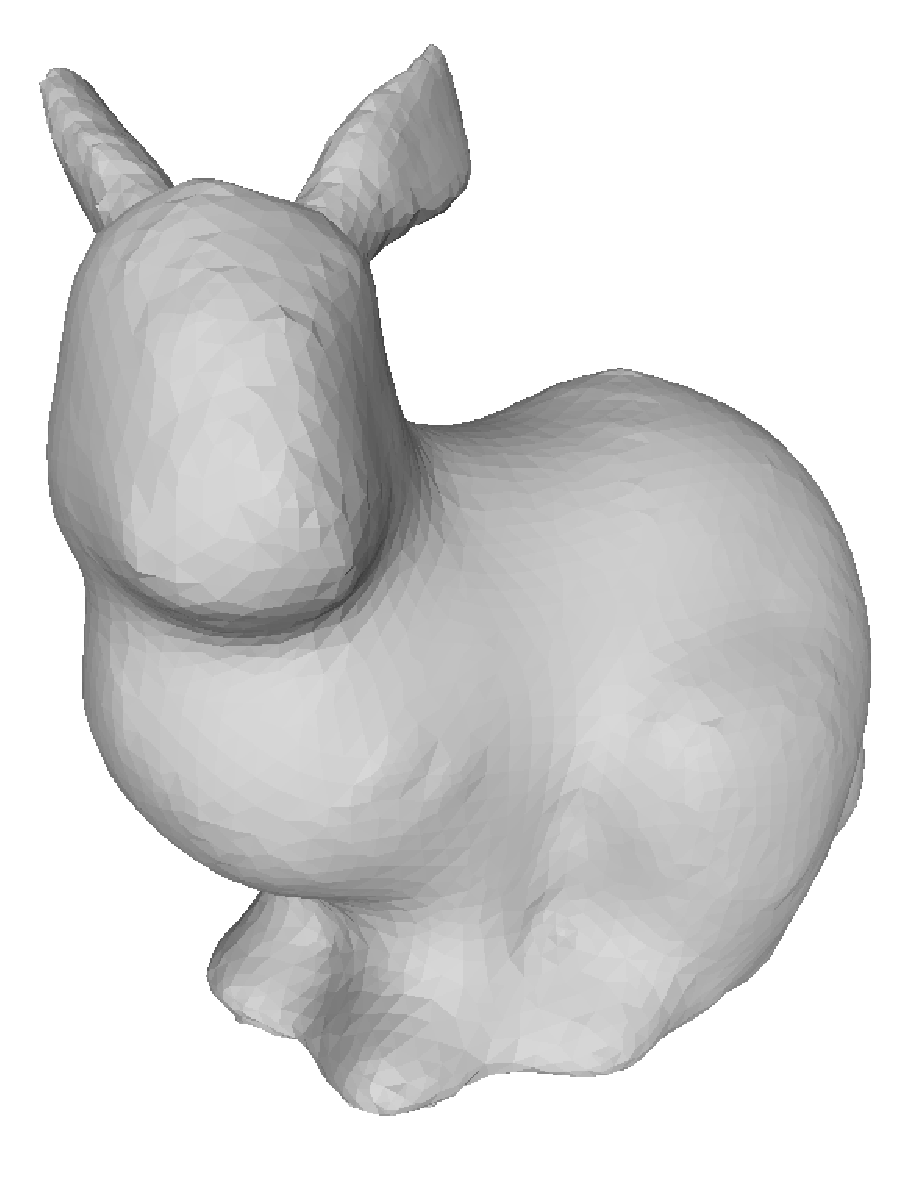
\includegraphics[width=\textwidth]{imagens/cap4/bunny_30.eps}
		\caption{30\% dos pontos}
		\label{fig:ex43}
	\end{subfigure}
	\hfill
	\begin{subfigure}[b]{0.47\textwidth}
		\centering
		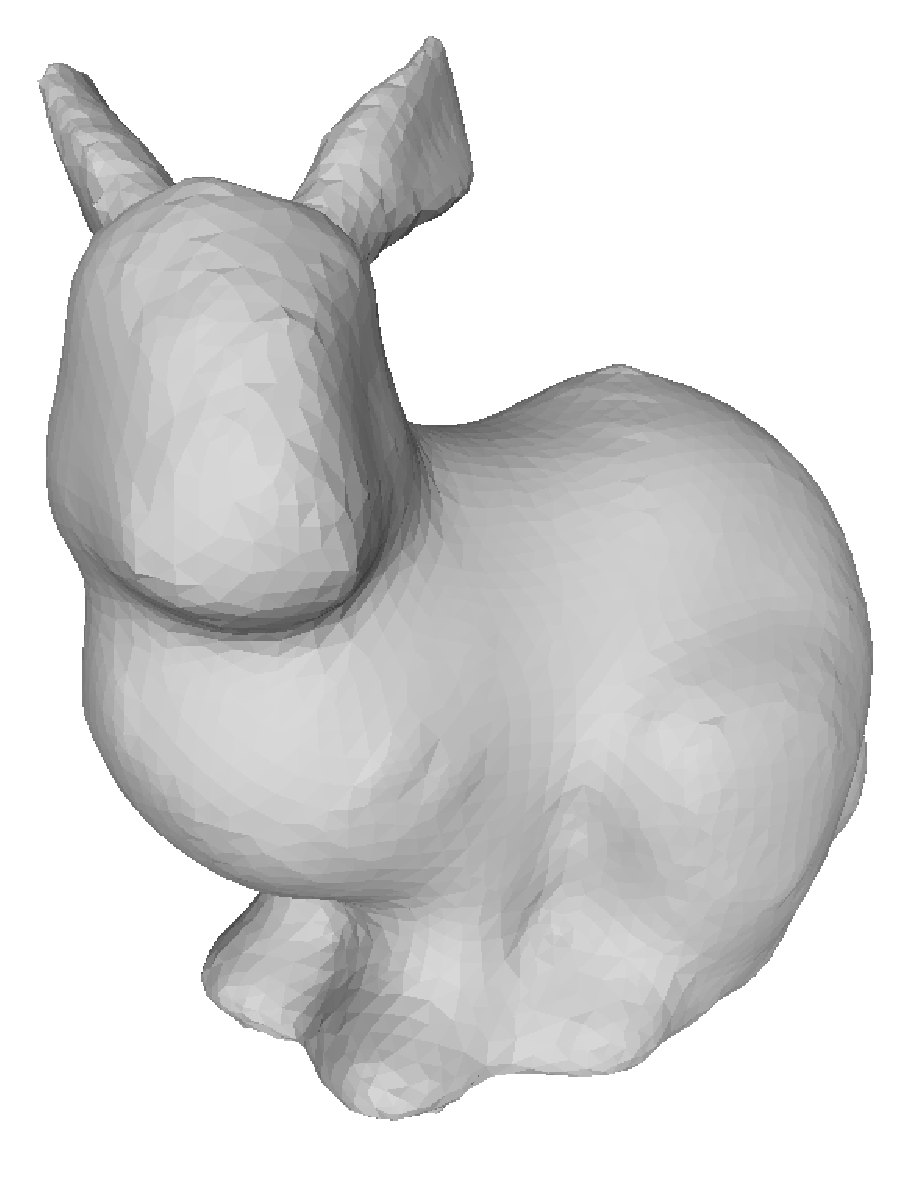
\includegraphics[width=\textwidth]{imagens/cap4/bunny_50.eps}
		\caption{50\% dos pontos}
		\label{fig:ex44}
	\end{subfigure}
	\caption{Representação da malha de um coelho, utilizando apenas uma amostra dos pontos originais como âncoras.}
	\label{fig:ex4rep}
\end{figure}


Nesta figura \ref{fig:ex4rep}, pode-se perceber que alguns detalhes visualmente impactantes do coelho (como o nariz e as pernas) são formados por poucos pontos, e que se estes não forem escolhidos como âncora, os detalhes podem ser perdidos.

\subsection{Edição de malhas}

Outra aplicação interessante das coordenadas diferenciais é a edição de malhas.

Para a edição de alguns vértices da malha, é feito algo similar à reconstrução mostrada anteriormente - porém, além dos pontos âncora, também serão adicionadas restrições dos vértices a serem editados.

Ou seja, além dos $m$ pontos $c = \{v_1, \dots, v_m\}$, são escolhidos $a$ pontos de índices $\{m+1, m+2, \dots, m+a\}$ denominados $e = \{v_{m+1}, v_{m+2}, \dots, v_{m+a}\}$ (novamente, por simplicidade, os pontos são indexados nas primeiras posições, logo após os pontos âncora), e adicionadas as restrições do tipo:

\begin{align}
\mathbf{v}_i &= \mathbf{c}_i, &i \in \{1, \dots, m\}\\
\mathbf{v}_j &= \mathbf{e}_j, &j \in \{m+1, \dots, m+a\}
\end{align}

\noindent e, matricialmente, o sistema pode ser escrito como:

\begin{equation}\label{eq:sisrecoveredi}
\left( \frac{L}{\omega I_{(m+a) \times (m+a)} | 0} \right) \mathbf{x'} = \begin{pmatrix}
\delta^{(x)}\\
\omega\ c_{1:m}^{(x)}\\
\omega\ e_{1:a}^{(x)}
\end{pmatrix}
\end{equation}

Ou seja, De forma gráfica, o sistema a ser resolvido para a edição pode ser visto como:

\begin{center}
	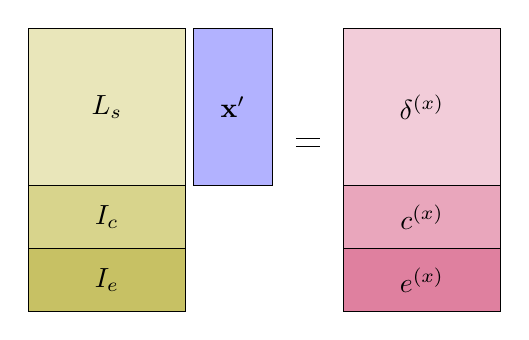
\begin{tikzpicture}
	\filldraw[fill=olive!20!white, draw=black] (0,0) rectangle node{$L_s$} (2,2);
	\filldraw[fill=olive!35!white, draw=black] (0,0) rectangle node{$I_c$} (2,-0.8);
	\filldraw[fill=olive!50!white, draw=black] (0,-0.8) rectangle node{$I_e$} (2,-1.6);
	\filldraw[fill=blue!30!white, draw=black] (2.1,0) rectangle node{$\mathbf{x'}$} (3.1,2);
	\draw (3.4, 0.50) -- (3.7, 0.50);
	\draw (3.4, 0.60) -- (3.7, 0.60);
	\filldraw[fill=purple!20!white, draw=black] (4,0) rectangle node{$\delta^{(x)}$} (6,2);
	\filldraw[fill=purple!35!white, draw=black] (4,0) rectangle node{$c^{(x)}$} (6,-0.8);
	\filldraw[fill=purple!50!white, draw=black] (4,-0.8) rectangle node{$e^{(x)}$} (6,-1.6);
	\end{tikzpicture}
\end{center}

Como é utilizado o método dos mínimos quadrados para a resolução dos sistemas, talvez aconteça alguns erros de precisão. Assim, para minimizar estas falhas, após se encontrar a solução do sistema, pode-se conferir alguns pontos (ou seja, o algoritmo pode, após encontrar os pontos pelo sistema, forçar com que $v'_i = v_i$, para alguns $i$, para que pelo menos estes pontos não sofram erros de precisão).

\begin{figure}[ht!]
	\centering
	\begin{subfigure}[b]{0.45\textwidth}
         \centering
         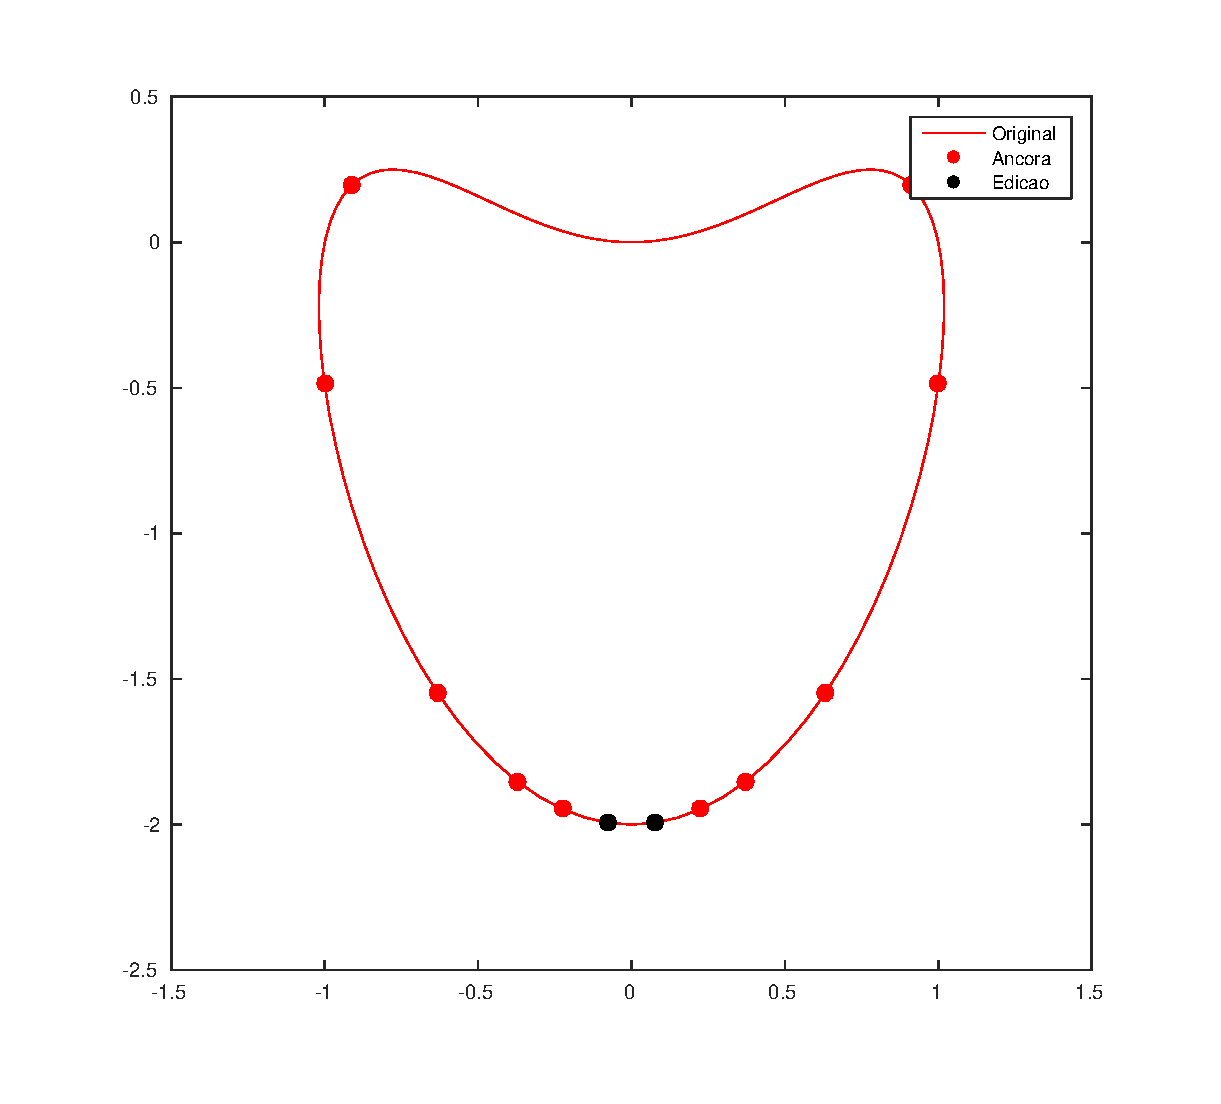
\includegraphics[width=\textwidth]{imagens/cap4/malhaoriginal.eps}
         \caption{Malha original}
         \label{fig:meshorigiedit}
     \end{subfigure}
     \hfill
     \begin{subfigure}[b]{0.45\textwidth}
         \centering
         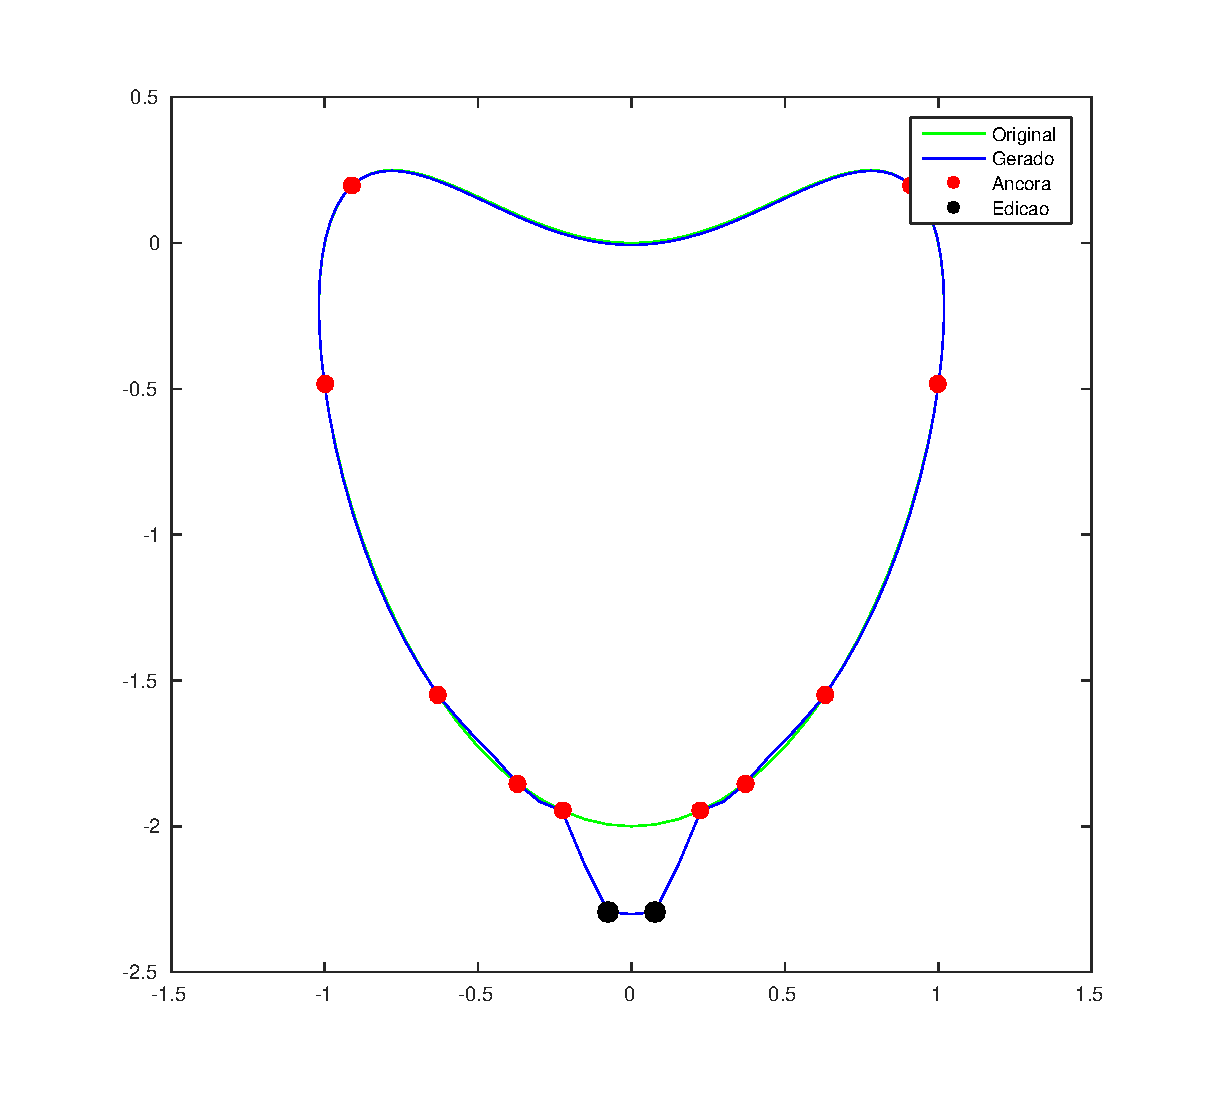
\includegraphics[width=\textwidth]{imagens/cap4/malhaedicao.eps}
         \caption{Malha editada}
         \label{fig:mesheditededit}
     \end{subfigure}
     \caption{Malha antes (\ref{fig:meshorigiedit}) e após edição (\ref{fig:mesheditededit}). Os pontos em vermelho são os pontos de âncora, e os pontos em preto são os editados.}
    \label{fig:editedmesh}
\end{figure}

Este processo pode ser aplicado em malhas tridimensionais, estendendo o sistema de duas $\delta$-coordenadas para três. Ou seja, através da resolução de mais um sistema similar ao exibido acima é possível editar malhas 3D através dos mesmos princípios utilizados para a edição de malhas 2D.  

Além de deformações, também é possível realizar outros tipos de edição, que são discutidas em \cite{sorkine2006}, como inserir marcas d'água, interpolar e suavizar malhas, que não serão discutidos neste livro.

